% Chapter 1

\chapter{Background} % Main chapter title

\label{Background} % For referencing the chapter elsewhere, use \ref{Background} 

\section{The Distributed Web}

\subsection{Blockchains}

\subsubsection{Introduction}
Since the 70's the modus operandi for data encapsulation and management has been SQL (Structured Query Languages) and RDBMS (Relational Database Management Systems). The 90's marked the arrival of the web, mass adoption of the Internet and networking of such database systems all over the world. However, because information is encapsulated in organisation centric forms, there are great inefficiencies communicating it over the network. Data sits in 'silos' and transferring it often requires an inevitable amount of bureaucracy and cost. In this context Blockchain technology offers an alternative approach to information storage. A global database that allows data to exists between organisations. So what are they? (see Vinay \cite{VinayOnBlockchains} for more on blockchains in context) \\

The concepts of a 'blockchain',  'blockchain technology' and 'distributed ledger technology' were first proposed and implemented by the Bitcoin electronic cash system, 2009\cite{nakamoto2008bitcoin}. The terms are used somewhat interchangeably to describe a peer to peer (and therefore decentralised) system that is capable of maintaining shared state in a way that is transparent, secure, permanent and resistant to corruption or attack. Within the Bitcoin cryptocurrency network, blockchains are used to maintain a globally consistent notion of account balances. There are now many more blockchain applications ranging from DNS registries (such as Namecoin\cite{Namecoin}) to alternative crypto currencies or 'altcoins' (such as LiteCoin\cite{Litecoin}, FairCoin\cite{Faircoin}, DogeCoin\cite{Dogecoin}) and even identity management systems (such as Onename\cite{Onename}). \\

The term blockchain is somewhat ambiguous in that it is often used interchangeably to describe both a data structure and a form of distributed database at the same time. A good description would perhaps make the distinction between a) a blockchain network - a peer to peer network that maintains distributed consensus on a blockchain data structure and b) a blockchain - the data structure that is stored by each peer (and therefore replicated across the entire network). Two things of important note are: Firstly the blockchain structure of the shared data is inextricable from the mechanisms used to maintain consensus of that data itself (this is a confusing statement that will be expanded upon shortly). Secondly, the comparison of blockchains to databases is conceptual. To be clear, a blockchain is not a relational database and there is no query language such as SQL. Further to this, sharding of blockchain data is uncommon in practise which is not generally the case in most other distributed database systems\cite{Shard}. \\

\begin{figure}
\centering
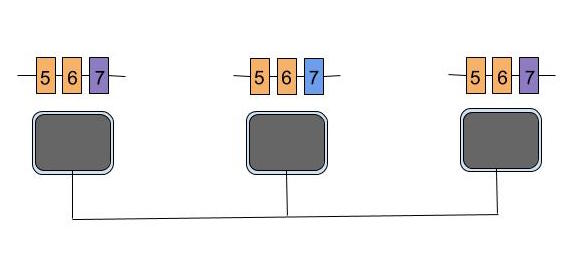
\includegraphics[width=\textwidth]{Figures/basic_chain}
\decoRule
\caption[Simplified Blockchain Network]{A simple illustration of a blockchain network with three peers.}
\label{fig:basic_chain}
\end{figure}

Figure \ref{fig:basic_chain} is an illustration of a simplified blockchain network. Each peer (grey box) has an almost identical full copy of the blockchain. Disagreement on final blocks is called 'forking'. Eventually all peers will agree on the same value for block 7. The type of consistency a blockchain network maintains is dependent on the number of blocks the observer chooses to discard from the end of the chain\cite{Bitcoin_consistency}. \\

\subsubsection{Transactions and Blocks}
Blockchain networks provide both read and write functionality. For the purposes of this discussion a transaction is a network input that results in a write to the blockchain. Whilst a read request may be fulfilled by any network peer, transactions must be processed by the entire network. For example, a payment in Bitcoin is a transaction. It causes a write to the blockchain as a change in account balances. \\

A block is a collection of transactions. The first block in a blockchain is called the genesis block. Each block thereafter represents a discrete update to the shared state. \\

\subsubsection{Blockchains as State Transition Systems}
A good approach to explaining blockchains is as state transition systems. State transition functions and finite state machines are familiar concepts to computer scientists. In a blockchain we can say that the history of the chain (i.e all previously processed transactions) encapsulates the state of the system. The addition of a new block, updates that history and therefore transitions the blockchain to a new state. This idea is illustrated in figure \ref{fig:blockchain_transition} \\

\begin{figure}
\centering
\makebox[\textwidth][c]{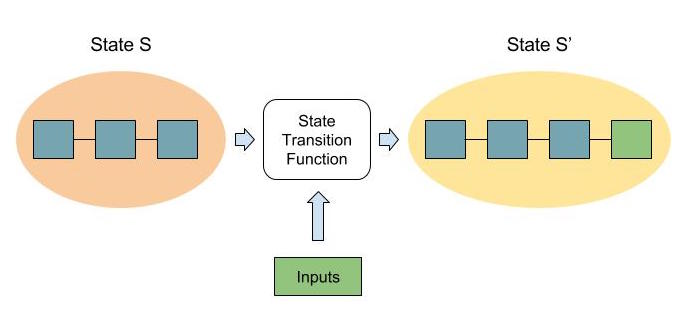
\includegraphics[width=1.4\textwidth]{Figures/blockchain_transition}}
\decoRule
\caption[Blockchain As State Transition]{Conceptualisation of a blockchain as a state transition system.}
\label{fig:blockchain_transition}
\end{figure}

The state may be encapsulated by the history of the blockchain in many ways. For instance, in the Bitcoin network the state is the sum of each user's unspent bitcoins i.e all account balances. A user's balance is derived by scanning through every previous block to find all received Bitcoins that have not yet been spent (users spend specific coins through the concept of unspent transaction outputs). This is not the case in the Ethereum network (discussed later) in which a user's balance is explicitly stored in every block (i.e no scanning operation required). An example state transition for a Bitcoin network is given in figure \ref{fig:bitcoin_transition}. There are five unspent transaction outputs in the initial state. The transaction uses two of these to make three payments. This results in a new state with six unspent transaction outputs. \\

\begin{figure}
\centering
\makebox[\textwidth][c]{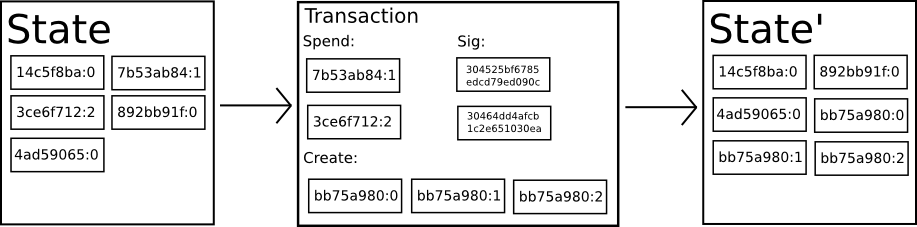
\includegraphics[width=1.4\textwidth]{Figures/state_transition}}
\decoRule
\caption[Bitcoin State Transition]{Bitcoin state transition diagram (taken from the Ethereum Whitepaper\cite{Ethereum})}
\label{fig:bitcoin_transition}
\end{figure}

The state transition function for a cryptocurrency like bitcoin might go something like:
\begin{enumerate}
\item Check each referenced or spent bitcoins (unspent transaction outputs) are available in the start state.
\item Check transaction signature is same as the bitcoin owner
\item Check sum of input bitcoins is at least equal to sum of output bitcoins.
\item Return new state 
\end{enumerate}

\subsubsection{Blockchain mining}
Mining is the process through which new blocks are created and distributed across the network. The general process proceeds something like the following:
\begin{enumerate}

\item A network peer creates or collects transactions (i.e state changing inputs).


\item A block header is created containing a number of fields. This includes the hash of the previous block (which creates a link in the chain), the block difficulty, a timestamp and a compressed, unique identifier, for the transaction set e.g a merkle\cite{Merkle} tree root.


\item The peer generates a proof of work. A typical proof of work involves repeatedly hashing\cite{Hash} the block header, varying a small amount of data each time (called the nonce) until a hash is produced with some agreed characteristics. One example is X amount of leading zeros (X is then the block difficulty).


\item The inputs (from step 1) and the block header (from step 2) form a block which is broadcast to the rest of the network. 


\item Peers receiving the block 

\begin{enumerate}
\item Check the hash of the previous block is valid

\item Validate the new state. Apply the block transactions to their current state (using the particular state transition function of the system) to check they are correct.

\item Add the block to their chain.
\end{enumerate}
\end{enumerate}

\begin{figure}
\centering
\makebox[\textwidth][c]{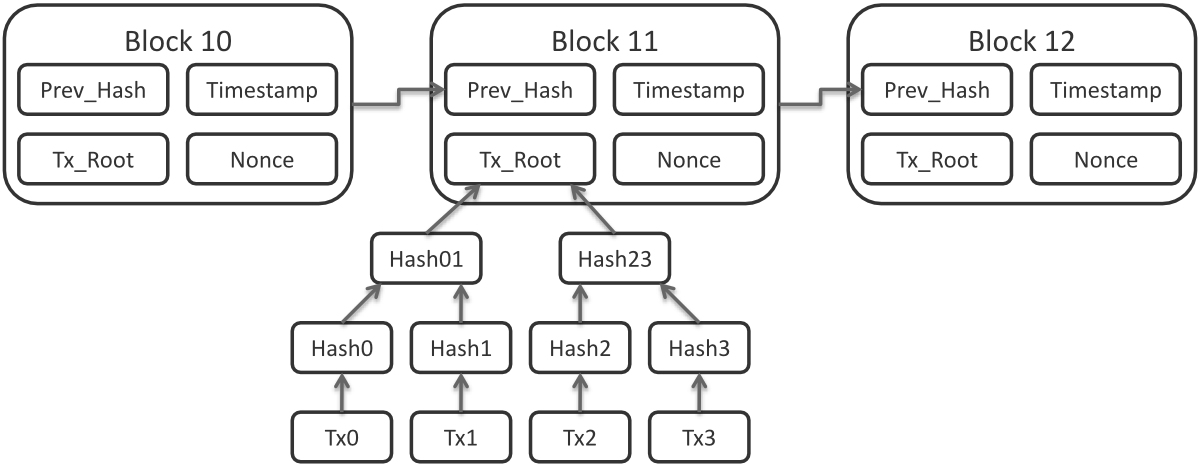
\includegraphics[width=1.4\textwidth]{Figures/blockchain}}
\decoRule
\caption[Sequence of Blockchain Headers]{A section of blockchain headers. Illustration by Matthaus Wander (Wikimedia) \cite{blockchainHeaders}}
\label{fig:bitcoin_transition}
\end{figure}

\subsubsection{Proof of work, hash functions and security}
The use of hash functions in both the compression of transactions in step 2 and the generation of a proof of work in step 3 are crucial to the security and consensus mechanisms of blockchain systems.\\

Any change to the input of a hash function results in a change in the output. Finding an input to a hash function that results in a given output is incredibly difficult and only achievable through a  brute force approach. This has two important implications.\\

Firstly, a proof of work (e.g generate hash with X leading zeros) can only be found through a trial and error approach. This establishes a formal economic barrier (electricity cost of CPU cycles) that limits the ability of any peer to add a new block to the chain. \\

Secondly, any change to a transaction in a previous block would result in a new transaction hash, which in turn would change the transaction root which in turn would change the block header. This would invalidate both the proof of work for that block and the previous hash link used in the next block. \\

This makes it impossible to change any transaction in the history of the chain without redoing the proof of work for every subsequent block. Such an undertaking is computationally infeasible for any group (colluding or otherwise) that cannot produce blocks faster than the rest of the network. In the case of most public blockchains this would require significant capital resource. \\

\subsubsection{Incentivisation} 
The maintenance of blockchain networks requires the incentivised participation of miners. Whilst this may not necessarily be economic, most public blockchain systems (including Bitcoin and Ethereum) have some form of mining reward and/or transaction fee to allow miners to collect a direct monetary reward for producing blocks.\\

\subsubsection{Forks and consensus}
When multiple blocks are produced in quick succession, network latency can cause the forking of blockchains. Figure \ref{fig:basic_chain} is a simple example of a fork. \\

At some point, one partition of the network will become aware of a longer chain being mined by another partition. Because this chain is longer, it contains a greater amount of work and is more likely to be accepted by the rest of the network. Miners are incentivised to work on the chain that is most likely to be adopted by the rest of the network because it increases the chance that their reward for creating blocks will be permanent.\\

\subsection{Ethereum}
\subsubsection{Introduction}
Ethereum is a public blockchain platform for running arbitrary applications with extremely low possibility of downtime, censorship, fraud or third party interference. It is a peer to peer network that stores turing complete programs within a blockchain. It has been described as a 'global computer' and a 'globally executed virtual machine'. The idea was first proposed by Vitalik Buterin who formally unveiled the project at the Miami Bitcoin Conference in early 2014. Later that year Ethereum is estimated to have raised over 20 million dollars in less than a month, making it one of the most successful crowdfunds ever\cite{Ethereum_crowdfund}. \\

The previous section of this report described how blockchains can be considered as state transition systems. The state transition function of Ethereum works by executing turing complete programs that are stored in the blockchain itself. In this sense it is perhaps the most general blockchain system conceivable. Bitcoin, Namecoin and Coloured Coins could all be implemented as contract code executing on the Ethereum blockchain. Buterin has described it as "The ultimate foundational layer"\cite{Ethereum}. \\

Although the state transition system may be very innovative, the fundamental consensus and proof of work mechanisms are very similar to other blockchain networks. The Ethereum platform still needs to incentivise miners and for this purpose has it's own internal cryptocurrency called Ether. \\

The rest of this subsection provides an introductory explanation to the Ethereum protocol. A more complete introduction has been written by Buterin\cite{Ethereum} and a comprehensive technical specification has been written by Wood\cite{wood2014ethereum}. Practical information and references for navigating the Ethereum ecosystem can be found in Appendix \ref{AppendixA}. \\

\subsubsection{Ethereum Accounts}
There are two types of accounts in Ethereum: \keyword{externally owned accounts} and \keyword{contract accounts}. \\

\begin{figure}
\centering
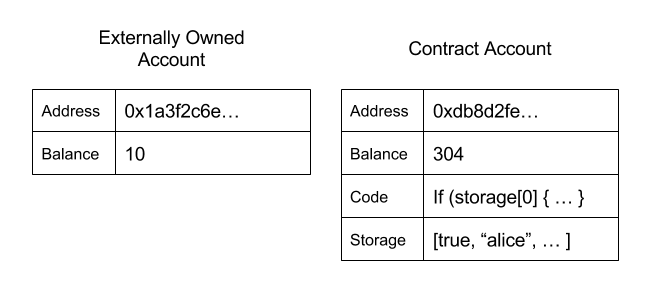
\includegraphics[width=\textwidth]{Figures/ethereum_accounts}
\decoRule
\caption[Ethereum Accounts]{Illustration of the two different types of Ethereum accounts}
\label{fig:ethereum_accounts}
\end{figure}

Externally owned accounts are effectively user accounts. They are controlled by private keys and have a balance in Ether. Contract accounts also have a balance but unlike externally owned accounts they also have code and storage. Contract accounts are controlled by their code. Both types of account are able to form transactions to both send Ether and call contract code.\\

\subsubsection{Ethereum as a state transition system}
Given this notion of accounts, the state of the Ethereum network is the aggregated state of each individual account. \\

Transactions are then either a) a direct transfer of ether between any pair of accounts, b) a contract creation request or c) a call to a contract method with a collection of argument parameters. Respectively, applying these transactions to the old state then either a) increases and decreases balances, b) adds a new account to the state or c) updates contract storage according to the execution of program code in the Ethereum virtual machine (EVM). \\

Unlike Bitcoin, where blocks simply contain a set of transactions, blocks in the Ethereum blockchain contain a copy of both the transaction list and the new state (balances, storage etc of all accounts). This account based approach, where the state is stored in every block, can seem more intuitive than that of unspent transaction outputs where state is derived through scanning the blockchain.\\

The consequence of storing the entire state in each block is that it is potentially inefficient in terms of storage. However, because most accounts do not change between blocks, a special type of merkle tree, called a patricia tree, is used so that data can be stored once and referenced multiple times ( a description of patricia trees is beyond the scope of this report but the interested reader should consult the Ethereum wiki \cite{Patricia}).\\

\begin{figure}
\centering
\makebox[\textwidth][c]{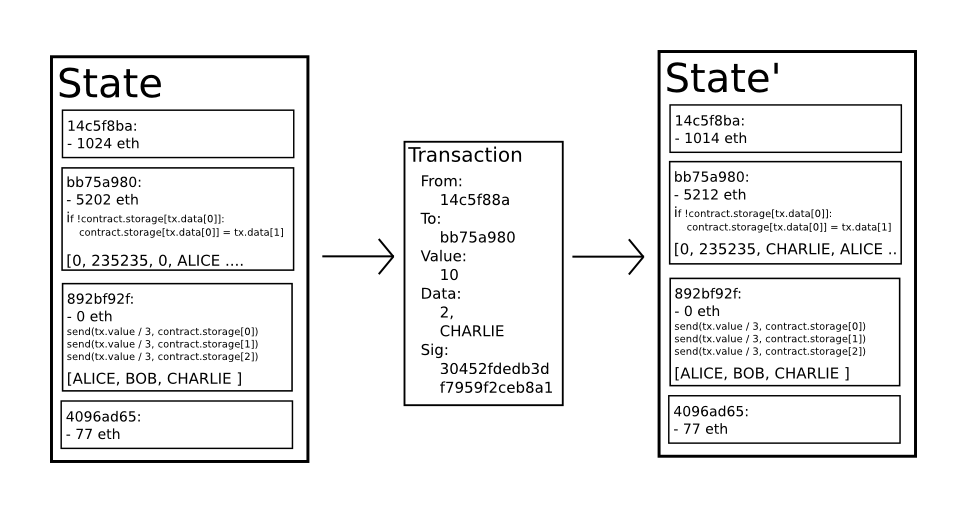
\includegraphics[width=1.2\textwidth]{Figures/ethereum_transition}}
\decoRule
\caption[Ethereum State Transition Diagram]{Ethereum State Transition Diagram (image taken from Etheruem Whitepaper\cite{Ethereum}).}
\label{fig:ethereum_transition}
\end{figure}

Figure \ref{fig:ethereum_transition} shows an example state transition in the Ethereum blockchain. The initial state contains four accounts; two externally owned (user) accounts and two contract accounts. The transaction is a call from the first user account to execute code in the first contract account with the arguments 2 and CHARLIE and an ether value of 10. In the resultant state, the balance of the user account has decreased by 10, the balance of the contract account has increased by 10 and the storage of the contract account has changed according to the execution of its code with the given arguments.\\

\subsubsection{Gas}
Any Ethereum transaction contains a STARTGAS and GASPRICE parameter. Startgas specifies a limit to the number of computational steps the sender is willing to pay for during code execution. The gasprice specifies the amount, in wei (a sub denomination of ether), they are willing to pay for each unit of computation. Unlike some other blockchain networks, transactions in Ethereum consume different amounts of computational resources; consider a simple ether payment vs execution of a complex insurance contract. By making agents pays proportionally for the resources they consume it becomes impossible to form denial of service attacks via infinite looping (possible given turing completeness of contract code). \\

The miner of a block collects the gas funds, therefore the gasprice functions in a similar way to transaction fees. The greater the gasprice the more incentive there is for a miner to include that transaction within a block. Any gas remaining after the execution of a transaction is returned to the sender.\\ 

\subsubsection{Blockchain Mining}
\begin{figure}
\centering
\makebox[\textwidth][c]{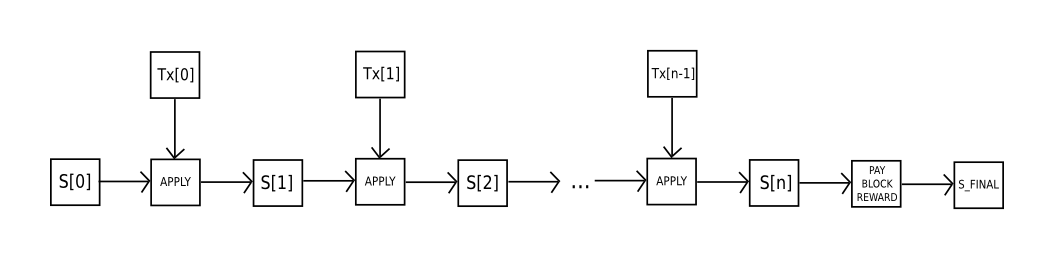
\includegraphics[width=1.2\textwidth]{Figures/ethereum_state_transition}}
\decoRule
\caption[Ethereum Block Validation Process]{Ethereum block validation process (image taken from Etheruem Whitepaper\cite{Ethereum}).}
\label{fig:ethereum_state_transition}
\end{figure}
The mining process of Ethereum is similar to the general blockchain process discussed in the previous section. The following steps describe the Ethereum block validation process as described in the Ethereum whitepaper (APPLY function executes transition function as above):

\begin{enumerate}
\item Check if the previous block referenced exists and is valid.


\item Check that the timestamp of the block is greater than that of the referenced previous block and less than 15 minutes into the future


\item Check that the block number, difficulty, transaction root, uncle root and gas limit (various low-level Ethereum-specific concepts) are valid.


\item Check that the proof of work on the block is valid.


\item Let S[0] be the state at the end of the previous block.


\item Let TX be the block's transaction list, with n transactions. For all i in 0...n-1, setS[i+1] = APPLY(S[i],TX[i]). If any application returns an error, or if the total gas consumed in the block up until this point exceeds the GAS LIMIT, return an error.


\item Let S\_FINAL be S[n], but adding the block reward paid to the miner.


\item Check if the Merkle tree root of the state S\_FINAL is equal to the final state root provided in the block header. If it is, the block is valid; otherwise, it is not valid.

\end{enumerate}

This process implies that every peer must eventually execute any contract code called by a transaction in order to check the validity of a new block. This is the reason Ethereum is often described as a 'globally executed virtual machine'.

\subsubsection{Smart Contracts}
In the context of Ethereum, programs stored in the blockchain are primarily referred to as smart contracts. Accounts that store code are called 'contract accounts'. The concept has a much broader definition outside of this context and was actually coined by Nick Szabo as early as 1993. According to Szabo "A smart contract is a computerized transaction protocol that executes the terms of a contract. The general objectives of smart contract design are to satisfy common contractual conditions (such as payment terms, liens, confidentiality, and even enforcement), minimize exceptions both malicious and accidental, and minimize the need for trusted intermediaries"\cite{SmartContract}. \\

It is easy to see how Ethereum contracts fall under this definition. However, the power of Ethereum code as 'smart contracts' is clearly limited to the clauses that can be meaningfully executed within the context of a blockchain.\\

The Ethereum Frontier guide\cite{Contracts_guide} suggests that contracts generally serve four purposes: \\

"\keyword{Contracts as data stores}. Examples include currencies, membership and registration. These are clear applications that can benefit from the transparency and incorruptibility of the block chain.\\


\keyword{Forwarding Contracts}. Code that is activated when certain conditions are met. This incorporates a very wide range of contracts because ?conditions? can be affected by many actors including organisations, individuals or even IOT devices. Multi signature accounts are a simple example of a forwarding contract. Forwarding contracts are particularly interesting because of the ability of contract accounts to call methods on other contract accounts.\\


\keyword{Ongoing contracts or relationships}. For example financial, escrow, insurance and bounty contracts. Bounty or open contracts give rewards when a verifiable solution or condition is somehow met. \\


\keyword{Library contracts}. Contracts that provide useful functionality to other contracts."\\


For space saving purposes, contract code is stored as EVM opcodes in a binary format. The most popular high level language for writing Ethereum contracts is Solidity\cite{Solidity}. Figure \ref{fig:Simplestorage} shows an example Solidity program. More information about the Solidity language can be found at the website - see ref.\\

\begin{figure}
\centering
\makebox[\textwidth][c]{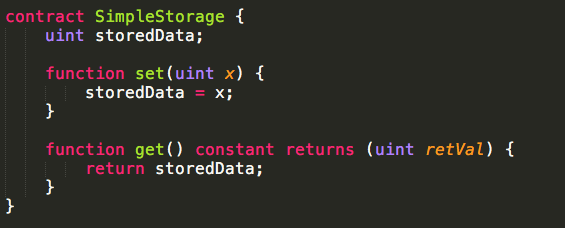
\includegraphics[width=1.4\textwidth]{Figures/Simplestorage}}
\decoRule
\caption[SimpleStorage Smart Contract]{An example Solidity smart contract called SimpleStorage.}
\label{fig:Simplestorage}
\end{figure}

\subsubsection{Dapps}
Dapp is short for distributed application. In the context of Ethereum a dapp is a complete application that incorporates not just a smart contract system (for executing something akin to server side logic) but also a client side user interface and any other architectural components. \\

Client side interfaces can be built with the same Javascript/HTML/CSS stack as normal web applications. It is common to see distributed filesystems such as IPFS (discussed in \ref{subsec:ipfs}) form part of dapp architectures. 

\subsubsection{Value Proposition}
The above description of Ethereum is fairly technical and esoteric. It is important to maintain sight of the purpose of such technology or, in the parlance of startup culture, the value proposition. The following question was raised at Ethereum DevCon1 during a panel on "The pathway to Ethereum adoption" \cite{devconvid}:\\

"I'm really excited about the potential of Ethereum to form the bedrock of a new socioeconomic paradigm. However, I'm not a developer, I'm not a dude, I don't work in bank, so I get the feeling you're baking a fatal flaw into this system at its inception by focusing on such a narrow demographic. What outreach plans do you have to encourage demand rather than focus on supply?".\\

The question highlights a misunderstanding about the value proposition of Ethereum. Unlike some other blockchain systems, such as Bitcoin, Ethereum is intended as a tool for application developers, not as a platform for end users. The offer to developers is a computation platform that is highly available, secure and transparent, has authentication and payment built in and is highly interoperable. However, performance requirements and costs also mean that Ethereum is not suitable for every application. 

\subsection{The InterPlanetary File System}
\label{subsec:ipfs}
The Inter Planetary File System (IPFS) is a content addressed, versioned, peer to peer file system. It aims to enable the creation of completely distributed applications and to make the web faster, safer, and more open.\\

IPFS synthesises the innovations behind many projects including the Self-Certifying File System\cite{mazieres1998escaping}, Kademlia\cite{maymounkov2002kademlia} (distributed hash table), BitTorrent and Git to propose a new alternative web protocol. The motivation and technical specification for IPFS has been well articulated by Benet in both the IPFS white paper\cite{benet2014ipfs} and a seminar at Stanford university\cite{IPFSVid}.

\subsubsection{The Problems}
In his Stanford seminar Benet highlights many challenges faced by the current web infrastructure:\\
\\
\keyword{Bandwidth}\\
The bandwidth of the network is not increasing at a significant rate. \\
\\
\keyword{Usage}\\
Storage prices are decreasing at a faster rate than the price of bandwidth. At the same time the demand for large data content is increasing e.g video conferencing, high definition media, 360 video etc. The combination leaves the impression that the network is actually slowing down.\\
\\
\keyword{Demand}\\
More and more devices and global populace are coming online. Extra demand is placing more strain on the network. Lesser economically developed countries experience the highest levels of network latency.\\
\\
\keyword{Centralisation}\\
Most of the data we use is controlled and maintained by a handful of organisations. This makes the data susceptible to physical disasters\cite{DCFire} as well as digital attacks. Furthermore, distribution of content is inefficient as the same data is sent across the network hundreds, thousands or even millions of times.\\
\\
\keyword{Permanence}\\
Content is addressed by location. The consequence is that if content is moved the link is broken and if the server is simply taken down the content may be lots forever.\\
\\
\keyword{Censorship}\\
The centralisation of services makes it very easy to censor communication and information applications by controlling the gateways for nation or state internet connections. Totally in browser applications using distributed data in peer to peer networks are resilient to weak links.\\
\\
\keyword{Resilience}\\
Whilst less severe than censorship, ISP outages and internet breakages are still a practical concern. The server client asymmetry makes it difficult for users to communicate and share data on a local area network when disconnected from the wider internet. \\
\\
\keyword{Control \& Security}\\
The transmission of data is typically secure but it is often stored in unencrypted formats both on the server and in the browser. \\

\subsubsection{The IPFS Solution}
\begin{figure}
\centering
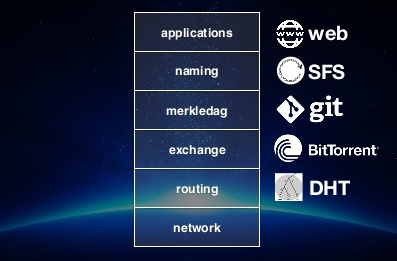
\includegraphics[width=\textwidth]{Figures/IpfsStack}
\decoRule
\caption[IPFS Stack]{The IPFS technology stack}
\label{fig:IpfsStack}
\end{figure}

Figure \ref{fig:IpfsStack} shows the various levels of, and contributions to, the IPFS stack. The core of IPFS is formed by the Merkle DAG (directed acylic graph). The IPFS Merkle DAG is a directed acyclic graph whose edges are merkle links. Essentially, this means that content can be addressed by a deterministic hash of the content itself i.e the root of a merkle tree structure. The use of merkledags, as with Git, also makes it possible to work offline first and version content. The properties that fall out from using Merkle DAG are that objects can be: a) retreived via their hash, b) integrity checked, c) linked to others and d) cached indefinitely. This all helps to make objects permanent. However, IPFS also implements a naming system, based on the work around self certifying file systems, that makes it possible to overlay the 'forest' of immutable objects with mutable links.\\ 

Distributed hash tables and block exchange peer to peer protocols build a sophisticated way to distribute and move the data (merkledags) as effectively as possible.

\section{Cooperative  Forms of Organisation}
\subsection{Brief History}
From the onset of  the industrial revolution a number cooperative and mutual responses emerged to the rapid growth of urbanisation, private companies and market mechanisms.  These include building societies, friendly societies, retail and wholesale cooperatives that aimed to provide services or benefits (access to housing, health care, out of work benefit, wholesome food etc) to defined communities of members.\\

\begin{figure}
\centering
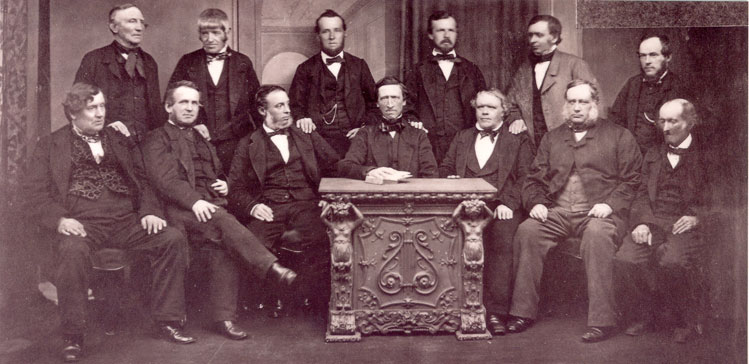
\includegraphics[width=\textwidth]{Figures/rochdale_pioneers}
\decoRule
\caption[Rochdale Pioneers]{The Rochdale Pioneers}
\label{fig:pioneers}
\end{figure}

The Rochdale Society of Equitable Pioneers, who formed in 1844\cite{Pioneers}, became the most successful and long lasting cooperative collective and are widely considered to be the founders of the modern cooperative movement. This is largely attributed to their documentation of cooperative principles\cite{Principles}, which established a values based organisational framework that subsequent cooperatives were able to adopt.\\

Throughout the rest of the century, many more cooperatives formed in the United Kingdom and independent movements also emerged elsewhere, such as credit unions in Germany and consumer cooperatives in the U.S.A. The colonial pursuits of European nations carried the cooperative model across the continents to India, Africa and South America where there remain strong cooperative communities to this day \cite{Coops_india_wiki}\cite{Coops_india}\cite{Kenya_coops}.\\   

In 1863, the Rochdale Pioneers merged with over 300 other cooperatives across Yorkshire and Lancashire to establish the North England Co-operative Society - which later became known as the CWS (Cooperative Wholesale Society). The CWS merged with more cooperatives throughout the 20th century and is recognisable on most UK high streets today as The Cooperative group.\\

\subsection{Principles Of Cooperation}
A brief summary of the seven principles of cooperation as defined by The International Cooperative Alliance\cite{ICA}, an adaption of the original principles defined by Rochdale Pioneers:\\

\begin{enumerate}
\item \keyword{Voluntary and Open Membership} \\ Co-operatives are voluntary organisations, open to all persons able to use their services and willing to accept the responsibilities of membership, without gender, social, racial, political or religious discrimination.

\item \keyword{Democratic Member Control} \\ Co-operatives are democratic organisations controlled by their members, who actively participate in setting their policies and making decisions. 

\item \keyword{Member Economic Participation} \\ Members contribute equitably to, and democratically control, the capital of their co-operative.

\item \keyword{Autonomy and Independence} \\ Co-operatives are autonomous, self-help organisations controlled by their members. Any terms always ensure the democratic control of the membership and maintain co-operative autonomy.

\item \keyword{Education, Training and Information} \\ Co-operatives provide education and training for their stakeholders and inform the general public - particularly young people and opinion leaders - about the nature and benefits of co-operation.

\item \keyword{Co-operation among Co-operatives} \\ Co-operatives serve their members most effectively and strengthen the co-operative movement by working together through local, national, regional and international structures.

\item \keyword{Concern for Community} \\ Co-operatives work for the sustainable development of their communities through policies approved by their members.

\end{enumerate}

\subsection{Scale}
A report carried out by CICOPA (The International Organisation of Industrial and Service Cooperatives) estimates that cooperatives employ almost 12\% of the entire working population of the G20 countries and that co-operative enterprises generate partial or full-time employment involving at least 250 million individuals worldwide, either in or within the scope of co-operatives \cite{roelants2014cooperatives}.\\

The UK cooperative sector turned over 37 Billion in 2015\cite{Cooperative_economy}. In Denmark consumer co-operatives in 2007 held 36.4\% of consumer retail market (source: Coop Norden AB Annual Report 2007). In Japan, the agricultural co-operatives report outputs of USD 90 billion with 91\% of all Japanese farmers in membership (Source: Co-op 2007 Facts \& Figures, Japanese Consumers' Co-operative Union.). In Malaysia, 6.78 million people or 27\% of the total population are members of co-operatives (Source: Ministry of Entrepreneur and Co-operative Development, Department of Co-operative Development, Malaysia, Statistics 31 December 2009).\\

The cooperative movement involves millions of people and contributes to significant portions of the economy worldwide.\\

\subsection{Cooperative Forms}
Although all coops unite under one banner there are a variety of cooperative forms depending on which group of stakeholders constitute the membership. The main types of cooperative forms include:\\\\
\keyword{Worker coops}\\
Employees of the business form the membership e.g Suma wholefoods\cite{Suma}.\\\\
\keyword{Consumer coops}\\
Members are consumers or customers who buy goods or services from their cooperative e.g The Cooperative group\cite{TheCoop}.\\\\
\keyword{Producer or Agricultural coops}\\
Many dairy farmers form producer coops. Members are producers who cooperate to make, market and sell their products.\\\\
\keyword{Multi stakeholder coops}\\
A hybrid form where multiple classes of membership coexist such as workers, producers and consumers.\\\\
\keyword{Housing coops}\\
Similar to a consumer coop. Members share ownership of residential property. \\


\subsection{Legal Incorporation \& Official Bodies}
Across the world cooperatives incorporate as legal entities in many different forms such as charities and limited companies. Whilst some countries, such as the UK, have legislation that legally acknowledge cooperative forms of organisation (The Co-operative and Community Benefit Societies Act 2014\cite{CoopAct}), many countries do not.\\

Although not always a legal requirement most cooperatives have a set of documents that outline their specific governance processes. Such documents are often required to register with official bodies, such as Co-operatives UK\cite{CoopsUK}. Measuring the commitment to the cooperative principles is somewhat subjective and these official bodies fulfil a role of authority on cooperative identity.

\subsection{The Cooperative Movement Today}
\keyword{The Cooperative group in the UK}\\
In 2014 the Cooperative Group, one of the largest cooperatives both in the UK and in the world, reported billions of pounds in losses. Former city minister Paul Myners was commissioned to run an independent investigation into the crisis and concluded that it was essentially caused by serious problems of incompetence, stemming from the group's governance structures. \\

The Co-op voted in favour of Myners proposed reforms in 2014 and more recently have appointed Mike Bracken, the former Government Chief Data Officer and Executive Director of Digital, who has been celebrated for bringing agile processes into government\cite{AgileGov}, as their new digital officer\cite{bracken}. It remains to be seen how the Cooperative group will develop under it's new structure and with it's new digital direction but it undoubtedly faces twin challenges of both maintaining cooperative organisation and developing member participation at scale.\\
\\
\keyword{Open coops}\\
There is an emergent notion of an 'open coop' that combines best practices from both the cooperative and open source movements\cite{OpenCoop}. Definitions of 'open coops' also specify a commitment to the organisation and co-production of the commons on a global basis (see ref). The requirement for these new cooperative definitions can be understood as a product of the web which is a) creating digital and tech coops who are naturally aligned with open source values and b) eroding the geographical and national boundaries previously limiting cooperative activity.\\
\\
\keyword{Platform Coops}\\
Another emergent notion is that of platform cooperatives\cite{PlatformCoop}. The case made by its proponents\cite{TreborPC} is that internet platforms (such as Uber, Airbnb, Taskrabbit etc), that form the basis of the 'sharing economy', are very good at sharing the risk (e.g cars, houses, maintenance, insurance), which is externalised to the platform users, but not very good at sharing the platform itself. The value creators for big Internet platforms (e.g drivers, hosts, cleaners, content creators) have little or no democratic voice and suffer by the extractive nature of the 'middleman' role played by the platform.\\

Whilst the benefits of platform based services are readily identified\cite{TreborPC} (rise of freelance work, building of real social networks, service over ownership, quality control or accountability through reputation systems) the argument is that the nature of employment is often precarious, undemocratic and insecure. \\

The proposed solution, is to takeover and rebuild platform services as cooperatives. Such platforms would provide all the same benefits but improve worker and stakeholder relationships.\\
 
The idea is growing in popularity. There are already a number of platform cooperatives forming (Fairmondo\cite{Fairmondo}, Resonate\cite{Resonate}) and many events and gatherings have been organised.\\

\section{Related Work}
\label{subsec:RelatedWork}
\subsection{Loomio}
Loomio\cite{Loomio} is a web application that assists groups with collective decision making processes. Loomio is a cooperative social enterprise that has been 'incubated' by the Enspiral network\cite{Enspiral-loomio}. Enspiral has been described as the best working example of an open cooperative\cite{Enspiral}.\\

\subsection{Boardroom}
\label{subsec:boardroom}
Boardroom is a decentralised governance application being developed on Ethereum that allows users to create organisational boards that can add or remove members, elect a chair, create subcommittees and allocate budgets. By using Ethereum, Boardroom adds a layer of security, auditability and transparency to help the governance processes of most traditional business architectures. Boardroom also takes advantage of the interoperability of the Ethereum ecosystem and has an extendable plugin architecture to facilitate the use of other Ethereum applications such as  crowdfunders, prediction markets etc.\\

\subsection{DigixDAO and The DAO}
\label{subsec:DAOs}
DAO stands for decentralised autonomous organisation. There has been a lot of speculation about the propensity of the Ethereum platform to host DAOs as well as how successful such projects might be. According to Vitalik Buterin, creator of the Ethereum platform, a DAO "is an entity that lives on the internet and exists autonomously, but also heavily relies on hiring individuals to perform certain tasks that the automaton itself cannot do."\cite{DAOBlog} DAOs have internal capital that it is able to spend and use to reward certain activities. \\ 

This year saw the launch of two DAOs on Ethereum. The DigixDAO\cite{Digix}, a platform for trading gold backed tokens, reached it's goal of \$5.5 million in under 12 hours in March\cite{DigixCrowd}. TheDAO\cite{TheDAO}, which is essentially a public investment fund where members can vote on proposals and subcontract work, is estimated to have raised over \$120 million in May which would make it the most successful crowd fund ever\cite{DAOCrowd}.\\

Given the arrival of DAOs, it is interesting to consider the concept of a Decentralised Autonomous Cooperative.\\

\subsection{Robin Hood Asset Management}
\label{subsec:RobinHood}
The Robin Hood Coop (RHC)\cite{RHC} are a hedge fund organised as a cooperative. Compared to the majority of other hedge funds the RHC operates at 'ridiculously' low costs and uses a 'parasite' algorithm that copies the behaviour of the most successful traders on the market. The profit generated by RHC investments is invested into projects that are building 'the commons'. \\

In their April newsletter, RHC announced the launch of a new innovation "a share \& member management system on the Ethereum blockchain". The newsletter is scant on details but the acknowledgment of Ethereum's potential utility by cooperative enterprises is a welcome validation of this study. 

\subsection{BuyCo.io}
\label{subsec:buyco}
BuyCo.io is a 'collaborative purchasing toolkit' that aims to leverage blockchain technology to make it easier for businesses and individuals to join together and form buying or purchase cooperatives. "Traditionally, buying cooperatives are time and labour intensive to set up and run. BuyCo.io allows you to set one up in seconds with ordering, supplier management, governance, escrow and payment processing all fully automated."\cite{BuyCo} Buyco claim that by using blockchain technology they are able to provide greater levels of user control and faster transaction times at much lower costs than traditional e-commerce platforms. The project is currently in the proof of concept stage. The BuyCo whitepaper can be found on their website (see ref). \\

Both BuyCo and the Robin Hood Coop are likely to face similar design and implementation challenges to those explored in this study. Future work in this area would benefit from the input of these projects and collaboration between the many emerging cooperative based approaches to blockchain technology.



